% --- Marks ---
% !TeX program = xelatex
% UI-Thesis v1.0

% --- Template maker CopyRight ---
% این قالب بر اساس فرمت پایان‌نامه‌ها و رساله‌های تحصیلات تکمیلی دانشگاه اصفهان تهیه شده است.
% علیرضا روحی-دانشجوی دکتری گروه مهندسی نرم افزار دانشگاه اصفهان
% 1395
% rouhi.ir@gmail.com
% توصیه می‌شود که از توزیع تک‌لایو (TexLive2015) به بعد استفاده شود:
% http://tug.org/texlive/acquire-iso.html

% موفق باشید.
% با تشکر از امین فخاری که قالب اصلی این پایان نامه را برای دانشگاه صنعتی اصفهان تهیه نموده اند.
% 1395
% a101.fakhari@gmail.com

% --- Preamble ---
\documentclass[a4paper,fleqn,11pt,oneside]{book}
\usepackage{tikz}
\usetikzlibrary{arrows,shapes}

% --- Packages ---
\usepackage{Settings/UI-Thesis}
\usepackage{acronym}
\usepackage{multirow}

% --- Cross-reference commands ---
\theoremstyle{plain}
\newtheorem*{trick}{ترفند}

\newcommand{\xs}[1]{بخش~\ref{#1}}
\newcommand{\xc}[1]{فصل~\ref{#1}}
\newcommand{\xp}[1]{صفحه~\pageref{#1}}
\newcommand{\xf}[1]{شکل~\ref{#1}}
\newcommand{\xt}[1]{جدول~\ref{#1}}
\newcommand{\xa}[1]{پیوست~\ref{#1}}
\newcommand{\xd}[1]{تعریف~\ref{#1}}
\newcommand{\xr}[1]{قانون~\ref{#1}}
\newcommand{\xra}[1]{R~\ref{#1}}
\newcommand{\xl}[1]{کد~\ref{#1}}
\newcommand{\xal}[1]{الگوریتم~\ref{#1}}
\newcommand{\xe}[1]{معادله~\eqref{#1}}
\newcommand{\xex}[1]{مثال~\ref{#1}}
\newcommand{\xeq}[1]{رابطه~\eqref{#1}}

\newcommand{\mylr}[1]{\texorpdfstring{\lr{#1}}{#1}}
\eqenvironment{نکات}{itemize}
\eqenvironment{تعریف}{definition}
\eqcommand{مورد}{item}

\algnewcommand\algorithmicforeach{\textbf{for each}}
\algdef{S}[FOR]{ForEach}[1]{\algorithmicforeach\ #1\ \algorithmicdo}

\newcommand*\diamondarrow{%
  \stackengine{0pt}{\hspace{1.2ex}$\rightarrow$}{$\lozenge$}{O}{l}{F}{F}{L}}
\newcommand*\fdiamondarrow{%
  \stackengine{0pt}{\hspace{1.2ex}$\rightarrow$}{$\blacklozenge$}{O}{l}{F}{F}{L}}
\newcommand*\dltriangle{%
  \stackengine{0pt}{${-}{-}$}{\hspace{3.2ex}$\vartriangleright$}{O}{l}{F}{F}{L}}
\newcommand*\ltriangle{%
  \stackengine{0pt}{${-}$\hspace{-.5ex}${-}$}{\hspace{2.8ex}$\vartriangleright$}{O}{l}{F}{F}{L}}

\makeatletter
\providecommand*{\cupdot}{%
  \mathbin{%
    \mathpalette\@cupdot{}%
  }%
}
\newcommand*{\@cupdot}[2]{%
  \ooalign{%
    $\m@th#1\cup$\cr
    \hidewidth$\m@th#1\cdot$\hidewidth
  }%
}
\makeatother

% --- Colors and Sets ---
\lstset{escapeinside={/*@}{@*/}}
\definecolor{codebackground}{RGB}{255,255,255}
\definecolor{commentcolor}{RGB}{77,153,153}
\definecolor{keywordcolor}{RGB}{153,77,153}
\lstset{backgroundcolor=\color{codebackground}}

\lstset{
  captionpos=b,
  numberstyle=\tiny,
  %basicstyle=\ttfamily\footnotesize,
  %basicstyle=\setLTR\thefootnotesize\ttfamily,
  basicstyle=\setLTR\bfseries\fontsize{8.5pt}{0}\selectfont\ttfamily,
  columns=flexible,
  tabsize=2,
  numbers=none, %left,
  nolol=true,
  keywordstyle=\color{keywordcolor},
  commentstyle=\color{commentcolor},
  stringstyle=\color{blue},
  captiondirection=RTL,
  upquote=true,
}

\def\lstlistingname{کد}

% --- Document ---
\begin{document}

% === Style ===
\pagestyle{plain}
\pagenumbering{harfi}

% === In the name of Allah page ===
\clearpage
\thispagestyle{empty}
\newgeometry{left=3.5cm, right=3.5cm, top=3.5cm, bottom=3.5cm}
\begin{figure}
  \centering

\includegraphics[width = \linewidth]{Settings/Allah.png}
\end{figure}

% === Title page ===
\DepartmentFa{دانشکده مهندسی کامپیوتر}
\GroupFa{گروه فناوری اطلاعات}
\ThesisTypeFa{پروژه}
\DegreeFa{کارشناسی ارشد}
\FieldFa{فناوری اطلاعات}
\BranchFa{تجارت الکترونیکی}
\YourFullnameFa{***}
\FirstSupervisorFa{***}
\YearFa{تیر 1400}
\TitleFa{بازی‌وارسازی در مدیریت منابع انسانی}
\MakeTitlePage

% === Persian Abstract ===
% !TEX root = ../gamification-in-human-resource-management.tex
% !TeX program = xelatex


\AbstractFa{
در سازمان‌ها مشکلاتی نسبت به روحیه کارمندان وجود دارد، طوری که افراد اوقات بدی را در محل کار سپری می‌کنند و به خاطر محیط کار خشک، در زندگی شخصیشان دچار عارضه‌های روانی مختلفی شده‌اند. هر نوع مشکلی که با روان افراد در ارتباط باشد روی انگیزه آن‌ها و به تبع روی عمل‌کردشان تاثیرگذار است. در این نوشتار با بهره‌گیری از روش‌های بازی‌وارسازی یا گیمیفیکیشن در فرایند مدیریت منابع انسانی سعی می‌شود محیط کار جذاب‌تری برای کارمندان آماده شود تا روحیه کارمندان بهبود یابد و عمل‌کرد بهتری داشته باشند.
}

\KeywordsFa{
1- بازی‌وارسازی،
2- مدیریت منابع انسانی،
3- مدیریت،
4- بازی،
5- منابع انسانی
}
\MakeFarsiAbstract

% === Table of Contents/Figures/Tables ===
\setcounter{page}{0}
% \MakeTableOfContents
% \MakeListOfFigures
% \MakeListOfTables
% \MakeListOfAlgorithms

% === Re-Style ===
\clearpage
\pagestyle{myheadings}
\pagenumbering{arabic}
\setcounter{page}{1}

% === Chapters ===
\clearpage
\baselineskip=0.9cm
\setcounter{footnote}{0}
% !TEX root = ../gamification-in-human-resource-management.tex
% !TeX program = xelatex
\chapter{مقدمه}
\section{پیش‌گفتار}
زمانی که بتوانیم خشکی محیط کار را از بین ببریم، می‌توانیم انگیزه‌های فراوانی در کارمندان و منابع انسانی یک سازمان ایجاد کنیم؛ بازی‌وارسازی\LTRfootnote{Gamification} به دنبال ایجاد همین قابلیت است. بازی‌وارسازی در اصل یک علم برای ایجاد روندهای بازی در دنیای واقعی است \cite{boudlaie}؛ به طور دقیق‌تر بازی‌وارسازی روشی است که در آن با استفاده از عناصر و المان‌های موجود در بازی‌ها دنیای واقعی را مشابه یک بازی در نظر می‌گیریم تا بتوانیم تجربه‌ای که بازی‌ها ایجاد می‌کنند را در دنیای واقعی نیز به دست آوریم.

بازی‌وارسازی در صنایع و کاربردهای مختلفی قابل استفاده است؛ کاربردهایی مثل مدیریت منابع انسانی، آموزش، بازاریابی، بهبود تجربه مشتری و غیره. در این مقاله به طور ویژه به کاربرد بازی‌وارسازی در مدیریت منابع انسانی پرداخته می‌شود.
\section{مفاهیم پایه}
برای آنکه بتوانیم دید بهتری نسبت به موضوع پیدا کنیم، باید بعضی از مفاهیم پایه موجود در مدیریت منابع انسانی و بازی‌وارسازی مطرح شوند.

برای بررسی کل فرایند مدیریت منابع انسانی باید پنج جنبه استخدام، مدیریت عمل‌کرد و مشارکت، آموزش و استعداد، مدیریت دانش و فرهنگ سازمانی مورد واکاوی قرار گیرند \cite{amiriamin}. در این‌صورت می‌توانیم با بررسی نقش بازی‌وارسازی در هر کدام از این جنبه‌ها به کاربرد نهایی بازی‌وارسازی در مدیریت منابع انسانی بپردازیم.

همانطور که حاتمی \cite{atoz} اشاره می‌کند، در بازی ما همیشه با نقش بازیکن برخورد داریم، به همین خاطر استفاده از لفظ \emph{کاربر} در مورد کسانی که می‌خواهیم برایشان بازی طراحی کنیم، درست نمی‌باشد؛ در ادامه نوشته به خاطر قراردادن مخاطب در دنیای بازی، از لفظ \emph{بازیکن} استفاده می‌شود. برای ایجاد بازی‌وارسازی در هر فرایندی، کار اصلی و نهایی ما طراحی بازی‌هایی برای بازیکن‌هاست.

بنابر مطالعات حاتمی \cite{atoz} بازیکن‌ها دسته‌بندی‌های مختلفی دارند. دسته‌بندی بازیکنان به این شکل است:
\subparagraph{دستاوردگرا}
این دسته از بازیکنان کسانی هستند که به دنبال ثبت رکورد، افزایش رتبه در جدول رده‌بندی و دریافت مدال‌ها و نشان‌های افتخار هستند و با بازیکنان دیگر کاری ندارند. این افراد شیفته پیروزی و برنده‌شدن هستند و برای مثال مدیران سازمان در این دسته قرار می‌گیرند.
\subparagraph{جستجوگر}‫
این افراد به دنبال کشف بازی، یافتن نقاط کور، پیداکردن جاذبه‌ها و رمزهای بازی و به طور کلی جستجوی در بازی حرکت می‌کنند. برای مثال افراد واحد تحقیق‌وتوسعه می‌توانند از این دسته باشند.
\subparagraph{معاشرت‌گرا}‫
کسانی هستند که جنبه اجتماعی بازی برای آن‌ها مهم است و بازی می‌کنند تا با دیگران ارتباط برقرار کنند. به نوعی این افراد از بازی برای یافتن نقاط مشترک خود با دیگران استفاده می‌کنند و چیزی که بازی را برای آن‌ها جذاب می‌کند خوش‌گذرانی با دیگران است. در یک سازمان کارمندان زیادی می‌توانند در این دسته قرار گیرند و چندان به موقعیت کاری مربوط نیست.
\subparagraph{قاتل}‫
قاتل‌ها کسانی هستند که به دنبال تسلط بر دیگران هستند. یک قاتل از پیروزی خود و شکست دیگری خوشحال می‌شود. رهبران سازمان در این دسته قرار می‌گیرند.

برای اینکه متوجه شویم چه بازی و فرایند بازی‌گونه‌ای برای هر کاربرد مناسب است باید بازیکن‌های بازی را شناسایی کنیم، مشخص کنیم از چه دسته‌ای هستند و یک بازی متناسب با دسته آن‌ها طراحی کنیم. علاوه بر نگاه به سازمان باید به جامعه‌ای که سازمان در آن قرار دارد نیز توجه کرد. در ایران دسته‌های قاتل و جستجوگر درصد بالایی از بازیکنان را در بر می‌گیرند در حالی که در غرب، معاشرت‌گرایان کثرت دارند و حدودا ۸۰ درصد جامعه را شامل می‌شوند \cite{atoz}.

طبق دسته‌بندی حاتمی \cite{atoz}، بازی و بازی‌وارسازی نیز انواع مختلفی دارد که در ادامه به آن‌ها می‌پردازیم.
\subparagraph{پنهان}‫
در این مدل، بازیکن متوجه نمی‌شود که در حال انجام یک بازی است. در حقیقت بازی از نگاه بازیکن مخفی شده‌است.
\subparagraph{ظاهر}‫
در این حالت بازیکن می‌داند که به انجام یک بازی می‌پردازد و نسبت به بازی عالم است.
\subparagraph{فیزیکی}‫
یک بازی (مثل بازی‌های رومیزی) می‌تواند بر مبنای عناصر فیزیکی طراحی شود و عناصر بازی قابل لمس باشند که به این بازی‌ها، بازی‌های فیزیکی گفته می‌شود. زمانی که در بازی‌وارسازی از بازی‌های فیزیکی استفاده شود، مدل فیزیکی رخ می‌دهد.
\subparagraph{دیجیتالی}‫
زمانی که بازی‌ها بر مبنای اپلیکیشن یا محتوای دیجیتالی توسعه داده شوند یک بازی دیجیتالی ساخته می‌شود که با استفاده از این بازی‌ها، مدل بازی‌وارسازی دیجیتالی به وجود می‌آید.

همچنین دو نوع دیگر نیز قابل ذکر است \cite{killer}:

\subparagraph{موردی}‫
در مدل موردی تنها در قسمت‌های خاصی از کاربرد مورد نظر از بازی‌وارسازی استفاده می‌شود.
\subparagraph{کامل}‫
در مدل کامل کل فضای کاربرد تحت تاثیر بازی‌وارسازی قرار می‌گیرد.

با شناخت انواع بازی و بازی‌وارسازی می‌توانیم به نحو بهینه‌ای از روش‌های بازی‌وارسازی در کاربردهای مختلف استفاده کنیم.

\section{بازی‌وارسازی در منابع انسانی}
در فرایند مدیریت منابع انسانی فعلی اشکالات بسیاری وجود دارد و در سازمان‌ها از هر روشی که بتواند این مشکلات را رفع کند، استقبال می‌شود. استخدام‌های سازمان‌ها به وضعیت مطلوب نزدیک نیست و بعضی از استخدام‌ها منجر به به‌کارگیری افراد ناشایست می‌شوند. کارمندان در محیط شرکت کسل هستند و انگیزه‌ای برای انجام کارها ندارند. جلسات به صورت بی‌نتیجه برگزار می‌شوند و اتلاف وقت بسیاری دارند. خود کارمندان نیز در زندگی خود با بیهودگی، افسردگی و پوچی در معنای زندگی مواجه هستند که بخشی از این مشکلات شخصی به خاطر محیط کاری نامطلوب به وجود می‌آیند. بازی‌وارسازی در مورد این مشکلات می‌تواند کمک‌کننده باشد و به این وسیله می‌توان محیط کاری را بهبود بخشید \cite{boudlaie}.

البته طبق مطالعات سایت مسترگیمیفیکیشن \cite{mrg} در استفاده از بازی‌وارسازی در محیط کاری، نگرانی‌هایی هم وجود دارد؛ مواردی مثل اینکه کارمندان درگیر بازی‌های بچگانه می‌شوند و بازی‌کردن برای چنین افرادی مناسب نیست! نکته اصلی در این رابطه این است که بازی‌وارسازی لزوما به معنی بازی‌کردن نیست؛ می‌توان صرفا از المان‌های بازی استفاده کرد. در فرهنگ متداول محیط کاری، متضاد کار، بازی است و برعکس؛ چنان‌که می‌شنویم افراد در گفتگوهای خود هنگامی که می‌خواهند بگویند شخصی از زیر کار فرار می‌کند، می‌گویند بازی می‌کند. بنابر همین نوع نگاه، مدیران نگران می‌شوند که هنگام استفاده از بازی‌وارسازی کارمندان از محیط کار دور می‌شوند و به تبع بهره‌وری آن‌ها کاهش می‌یابد؛ در حالی که متضاد کار و همچنین متضاد بازی، افسردگی است \cite{tedx}. در حقیقت کسی که کار یا بازی نمی‌کند، افسرده است و کسی که افسرده است نمی‌تواند بازی کند یا کار کند. در بازی‌وارسازی صرفا از بازی‌ها استفاده می‌شود تا کار جذاب شود نه اینکه افراد فعالیت اصلی خود را بازی‌کردن ببینند.

در بازی‌وارسازی باید به این نکته توجه کرد که از این روش باید با هدف افزایش بهره‌وری افراد طوری که خود افراد تمایل دارند، استفاده شود \cite{tedx}. در حقیقت بازی‌وارسازی نباید برای ایجاد نوعی اجبار برای کارمندان یا دیکته‌کردن موارد به آن‌ها استفاده شود تا افراد طوری که ما می‌خواهیم رفتار کنند!
نکته دیگر این است که اگرچه بازی‌وارسازی در مدیریت منابع انسانی می‌تواند کمک‌کننده باشد اما خطراتی هم دارد \cite{atoz}. ممکن است کارمندان نسبت به انجام بازی‌ها مشتاق نباشند و نسبت به تغییرات جبهه‌گیری کنند. در بسیاری از پیاده‌سازی‌های بازی‌وارسازی از تکنیک ارائه پاداش استفاده می‌شود در حالی که این تکنیک لزوما کاربردی نیست. گاهی کارمند به دنبال پاداش نیست \cite{mrg}! بنابر نظر حاتمی \cite{atoz} اگر از روش‌های بازی‌وارسازی به شکل مطلوب استفاده نشود، صدمات جبران‌ناپذیری به منابع انسانی سازمان وارد می‌شود؛ مثلا، یک پیاده‌سازی غلط از بازی‌وارسازی در سازمان‌ها برای پرداخت بی‌رویه پاداش یا اصلا استفاده غیر منطقی از المان‌های بازی‌وارسازی، می‌تواند منجر به افزایش توقع کارمندان شود که این مسئله در بلندمدت به خاطر عدم توانایی سازمان در برآورده‌کردن توقعات، انگیزه کارمندان نسبت به کار را حتی بیشتر از قبل کاهش می‌دهد. یک نمونه دیگر از پیاده‌سازی غلط بازی‌وارسازی هنگامی رخ می‌دهد که طراحان بازی، کارمندان را همانند کودکان در نظر می‌گیرند و شناخت درستی نسبت به جامعه بازیکنان ندارند که در این حالت بازی‌وارسازی نتیجه‌ای کاملا برعکس دارد.

\subsection{بازی فوتبال}
یکی از مثال‌ها برای توضیح بازی‌وارسازی در فرایند مدیریت منابع انسانی، بازی فوتبال است. در صنعت فوتبال بازیکن‌ها (ورزشکاران) عملا کارمندان یک باشگاه ورزشی هستند و خود بازی، کار آن‌ها حساب می‌شود. کار این کارمندان می‌تواند برای باشگاه امتیازاتی مثل جوایز مسابقات یا صعود در جدول رده‌بندی به ارمغان آورد.
به خاطر ماهیت این کار که در صنعت سرگرمی فعالیت می‌کند و بیشتر جنبه تفریحی دارد، بازی‌وارسازی به خوبی در این کار می‌تواند پیاده‌سازی شود و نتایج آن مشخص شود. چند مورد از پیاده‌سازی‌های مرتبط با عناصر بازی‌وارسازی در بازی فوتبال در ادامه بیان می‌شوند.
\subparagraph{بازخورد}‫\LTRfootnote{Feedback}
بازخورد یکی از عناصر بازی‌وارسازی است که در آن به بازیکن به شکل آنی بازخوردهایی ارائه می‌شود و او را از نتیجه تصمیماتش آگاه می‌کند \cite{atoz}. در بازی فوتبال پس از اتمام هر بازی، بازیکن‌ها از سمت مربیان و کارشناسان مورد ارزیابی قرار می‌گیرند و نمره‌هایی به آن‌ها اختصاص داده می‌شود یا به شکلی دیگر آمارهای مرتبط با بازیکن (مثل تعداد پاس‌های صحیح یا درصد خطا در بازپس‌گیری توپ) به اطلاع وی رسانده می‌شود. این روند نمره‌دهی و ارائه آمار که پیاده‌سازی عنصر بازخورد از مجموعه عناصر بازی‌وارسازی است، به بازیکنان کمک می‌کند از نتیجه تمرینات خود مطلع شوند، ضعف‌های خود را بیابند و بتوانند بهتر بازی کنند و از سمت دیگر امتیازدهی می‌تواند نقش مشوق را برای بازیکنان ایفا کند. به این شیوه بازیکن روش کارکردن بیشتر و بهتر را متوجه می‌شود و بهره‌وری وی افزایش می‌یابد.
\subparagraph{جدول برندگان}‫\LTRfootnote{Leader board}
جدول برندگان عنصری از بازی‌وارسازی است که بر اساس امتیازات بازیکنان به آن‌ها رتبه‌ای در جدول می‌دهد و به این شکل بازیکن می‌تواند خود را با دیگر بازیکنان مقایسه کند \cite{atoz}. در یک بازی فوتبال، انتخاب بازیکن هفته، ماه و سال، یکی از پیاده‌سازی‌های مرتبط با جدول برندگان است.
\subparagraph{تصمیم‌گیری}‫\LTRfootnote{Choice}
در یک بازی دو نوع هدف بلندمدت و کوتاه‌مدت وجود دارد که در هدف بلندمدت بازیکن سعی می‌کند آمارهای آنی خود را بهبود ببخشد در هدف بلندمدت بازیکن باید به یک نتیجه نهایی برسد. عنصر تصمیم‌گیری به این می‌پردازد که بازیکن در هر لحظه چگونه تصمیم‌گیری می‌کند و انتخاب او بین رسیدن به هدف بلندمدت و هدف کوتاه‌مدت کدامیک خواهد بود که گاهی این دو هدف در تعارض با یکدیگر قرار می‌گیرند \cite{atoz}. در بازی باید انتخاب‌های معناداری وجود داشته باشند تا بازیکن با تصمیم‌گیری درگیر شود و همین کار باعث ایجاد جذابیت برای بازی می‌شود. آمارهای شخصی بازیکنان و انتخاب به عنوان بازیکن برتر زمین به عنوان هدف‌های کوتاه‌مدت در مقابل مشارکت با دیگر بازیکنان برای بردن جام‌های مختلف توسط تیم و باشگاه به عنوان هدف‌های بلند مدت می‌توانند این انتخاب و تصمیم‌گیری را در بازی فوتبال ایجاد کنند.
\subparagraph{چالش}‫\LTRfootnote{Challenge}
عنصر چالش اشاره به چالش‌هایی دارد که بازی برای بازیکن تعیین می‌کند \cite{atoz}. مثلا دریبل‌زدن یا گل از طریق ضربه آزاد نوعی چالش است که در فوتبال وجود دارد.
\subparagraph{نشان}‫\LTRfootnote{Badge}
در ازای انجام چالش‌ها می‌توان به عنصر نشان رسید. وقتی بازیکنی کارهای خواسته‌شده را انجام می‌دهد، بازی به وی نشان افتخار می‌دهد \cite{atoz}. این نشان می‌تواند انگیزه بازیکن را برای ادامه بازی افزایش دهد؛ مثلا در فوتبال، دادن عنوان‌هایی مثل \emph{شوالیه} یا \emph{بیبی‌فیس قاتل} از سمت تماشاگران، نوعی از پیاده‌سازی این عنصر است.
\section{سناریوهای شکست}
اگر بازی‌وارسازی به خوبی پیاده و بازی به نحو مطلوب و اصولی طراحی نشود، شکست‌های بدی برای سازمان به وجود می‌آید. در ادامه چند سناریواز سایت مسترگیمیفیکیشن \cite{mrg} به عنوان مثال‌هایی برای پیاده‌سازی‌های غلط بازی‌وارسازی آورده شده‌اند.
\subsection{بررسی وب‌سایت توسط متقاضی و اعطای نشان به وی}
مدیریت یک سایت تمایل دارد که متقاضیان استخدام با مطالعه سایت اطلاعات بیشتری نسبت به محیط کار آینده خود و موقعیت شغلی که برای آن درخواست داده‌اند کسب کنند، به همین دلیل می‌خواهد از بازی‌وارسازی در فرایند استخدام استفاده کند تا متقاضیان را به مطالعه سایت ترغیب کند. پس سناریویی طراحی می‌کند که در آن متقاضی امتیازهایی برای مطالعه مطالب سایت به دست می‌آورد و بر اساس امتیازها به افراد نشان‌هایی اعطا می‌شود. به این شکل یک پیاده‌سازی از روش‌های بازی‌وارسازی ابداع می‌شود.

مشکل سناریو و پاداشی که داده می‌شود این است که هیچ ارتباطی با هدف کلی آن یعنی استخدام ندارد و نشان‌ها در این فرایند تاثیرگذار نیستند. به خاطر عدوم وجود ارتباط بین هدف و پاداش، بازیکن رغبتی به انجام بازی ندارد و در نتیجه شناخت متقاضی نسبت به شرکت محقق نمی‌شوند.
\subsection{استفاده از سیستم معرفی برای ایجاد مشارکت در کارمندان و افزایش بهره‌وری}
مدیریت سازمان به دنبال ایجاد ارتباط بین کارمندان فعلی و کارمندان آینده سازمان است و همچنین بین اعضای فعلی سازمان نیز مشارکتی ایجاد کند. برای همین از \emph{روش معرفی }استفاده می‌کند. روش معرفی سناریویی است که در آن اگر کارمند فعلی سازمان برای موقعیت‌های شغلی مورد نیاز مدیران فردی را معرفی کند و فرد معرفی‌شده انتخاب شود، به او امتیازهایی داده می‌شود.

مشکل این سناریو این است که کار و بازی از یکدیگر جدا شده‌اند. در صورت پیاده‌سازی این سناریو، کارمندان ترجیح می‌دهند دائم موقعیت‌های شغلی را رصد کنند تا بتوانند برای هر موقعیت شغلی یک فرد مفید را پیشنهاد دهند و این یعنی بیشتر زمان کارمند صرف بازی معرفی می‌شود. از سمت دیگر توقعاتی برای کارمند ایجاد می‌شود؛ مثل این که کسانی که امتیاز بالایی دارند توقع افزایش حقوق زیاد، پاداش و مرخصی‌های طولانی می‌شوند که منطقی نیست ولی به خاطر اینکه نسبت به دیگران امتیاز بالایی دارند، در ذهن خود نتیجه‌گیری می‌کنند که از دیگر کارمندان سازمان بهتر هستند پس در نتیجه مستحق دریافت جوایز کلانی هستند.
% !TEX root = ../gamification-in-human-resource-management.tex
% !TeX program = xelatex
\chapter{کارهای پیشین}
در این فصل به تفصیل در مورد چند پیاده‌سازی ساده و جذاب از سناریوهای موفق مرتبط با مدیریت منابع انسانی صحبت خواهد شد. آنچه که در ادامه مطالعه می‌کنید، بر اساس بخش‌های مختلف فرایند مدیریت منابع انسانی جدا شده‌است.
\section{استخدام}
در مورد استخدام باید به دنبال طراحی بازی‌هایی باشیم که دارای تم‌های اصلی استخدام باشد، تم‌های اصلی استخدام به ترتیب در ذیل آمده‌اند:
\begin{itemize}
	\item طراحی برنامه‌ریزی شغلی
	\item شناخت مهارت‌های شغلی
	\item سنجش نوآوری
	\item توسعه زیرساخت‌های فناوری سازمان
	\item ویژگی‌های فردی
	\item شناخت سرمایه روانشناسی
	\item شناخت سرمایه اجتماعی
	\item قدرت تطبیق‌پذیری با اهداف شغلی
\end{itemize}
\subsection{بیلبوردهای گوگل}
در سال 2004 گوگل\LTRfootnote{Google} در بزرگراه 101 سان‌فرانسیسکو\LTRfootnote{San Francisco} که محل تردد کارمندان شرکت‌های معروفی مثل سیسکو\LTRfootnote{Cisco}، اپل\LTRfootnote{Apple}، ای‌بی\LTRfootnote{eBay} و غیره می‌باشد، یک بیلبورد رمزآلود با نوشته‌ای روی آن که صرفا می‌گفت \textit{اولین عدد اول ده‌رقمی که در دنباله نپر یافت می‌شود دات کام} نصب کرد (\xf{fig:google}) که افراد کنجکاو را وامی‌داشت تا معمای آن را حل کند که پس از حل معما و مراجعه به سایت مورد نظر\LTRfootnote{7182818284.com}، فرد با فرم تقاضای استخدام در گوگل مواجه می‌شود \cite{eprimesolve}.

\begin{figure}[!htb]
	\centering
	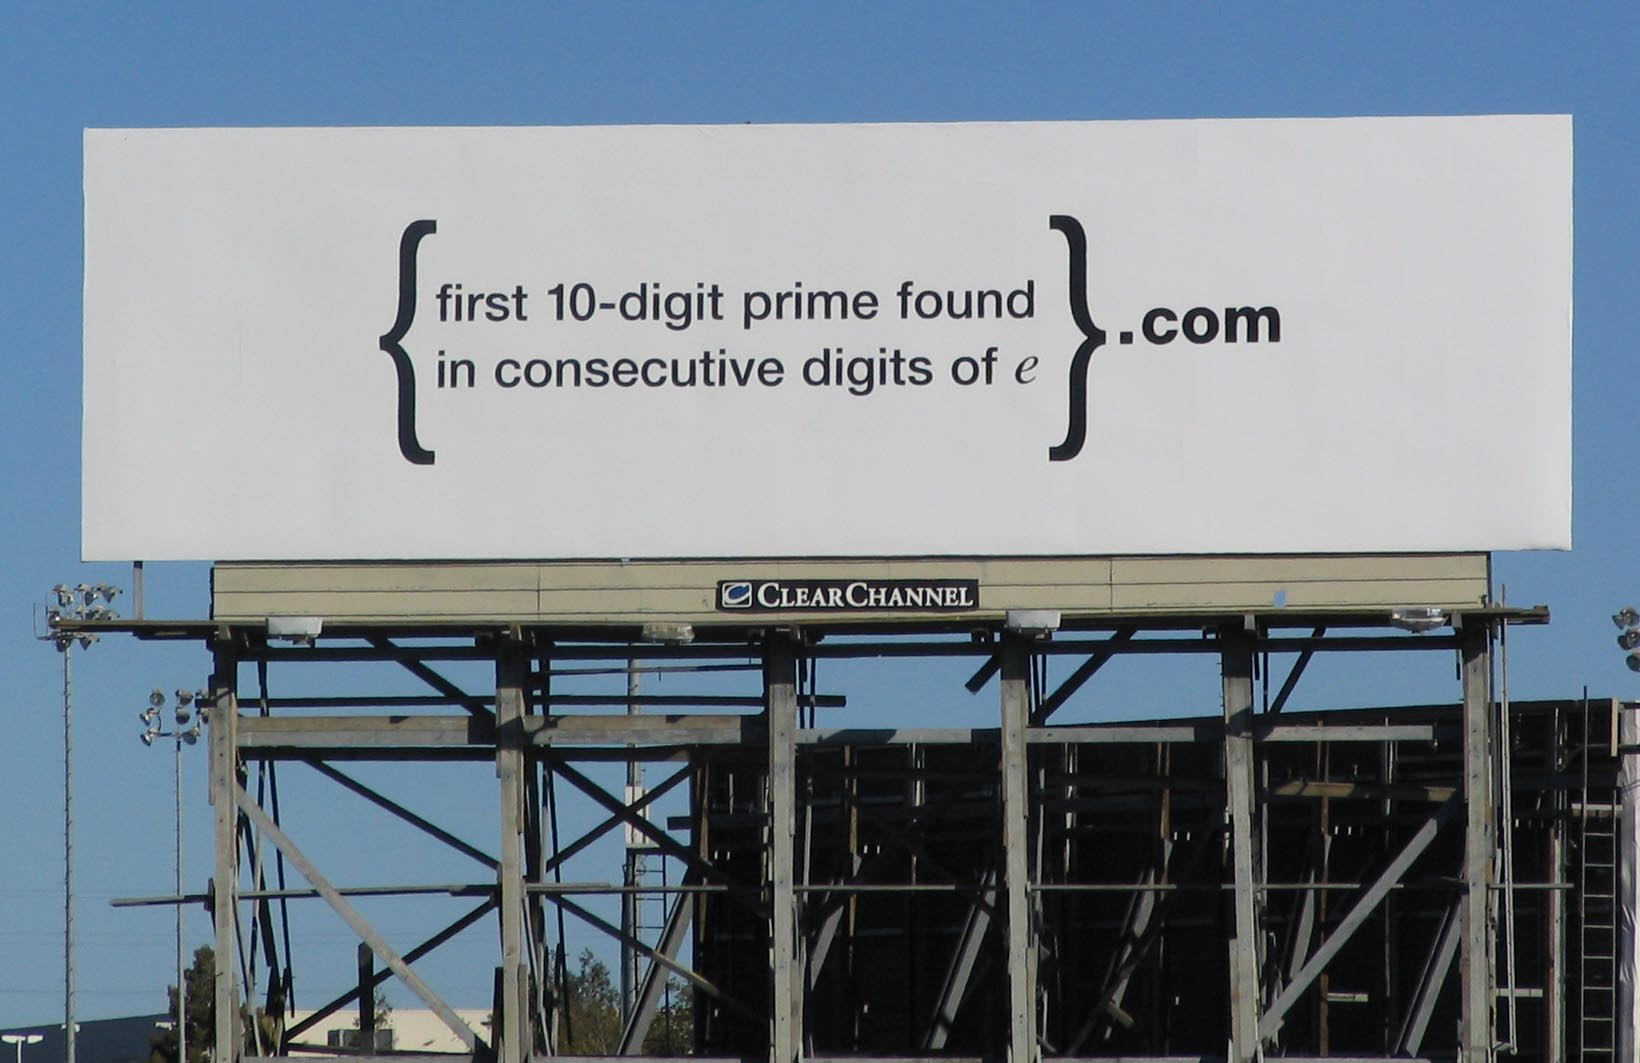
\includegraphics[width=\textwidth]{Figures/eprime.jpg}
	\caption{بازی استخدامی گوگل که با یک بیلبورد پیاده‌سازی شد\cite{eprimepic}}
	\label{fig:google}
\end{figure}


گوگل بدون آنکه اسمی از خود در این بیلبورد برده باشد، با کمک این معما و طراحی یک بازی توانست در فرایند استخدام خود به خوبی روندی گزینشی را طی کند. با این کار گوگل می‌توانست افراد کنجکاو (بازیکنان جستجوگر) و برنامه‌نویسانی با حداقل‌های لازم علمی و فنی را پیدا کند و خصوصیاتی که لازم داشت را بدون نیاز به صرف زمان، به دست آورد.

\subsection{ارتش آمریکا}
ارتش آمریکا بازی ویدیویی \href{https://www.americasarmy.com/}{\lr{America's Army}} را  در سبک شوتر اول‌شخص در سال 2002 برای عموم منتشر کرد. روش انجام بازی به این صورت است که افراد در گروه‌هایی چندنفره قرار می‌گیرند که یکی از اعضا به عنوان رهبر گروه، چند نفر نقش پشتیبانی و چند نفر سرباز گروه تعیین می‌شوند. گروه‌های مختلف به مبارزه با یکدیگر می‌پردازند و با در نظر گرفتن تاکتیک‌ها و نقشه‌هایی سعی می‌کنند گروه‌های دیگر را از بین ببرند \cite{eventful}.

این بازی علاوه بر تبلیغ ارتش آمریکا باعث شده‌است که علاقه‌مندان به حضور در ارتش با کمک این بازی بتوانند شناخت و تجربه‌ای بهتر نسبت به فضای ارتش و محیط نظامی کسب کنند و از سمت دیگر خود ارتش بهتر می‌تواند توانایی‌های ذهنی، اجتماعی فرماندهی و مهارتی افراد متقاضی را متوجه شود \cite{army}.

ارتش آمریکا همچنین از طریق بستر اشتراک ویدیوی آنی توییچ\LTRfootnote{Twitch live stream} به رصد بازیکنان می‌پردازد و افرادی را که مهارت‌های مورد نظر ارتش را دارند، جذب می‌کند \cite{uhl, cbs}. ارتش آمریکا از بستر بازی‌های ویدیویی برای افزایش مهارت‌های نرم و قدرت مشارکت تیمی نیز بهره می‌برد \cite{cbs}.

\subsection{قهرمان پیتزا دومینو}
امیری و امین \cite{amiriamin} در مقاله خود این مثال را مطرح کرده‌اند. پیتزا دومینو بازی جذابی با نام قهرمان پیتزا دومینو\LTRfootnote{Domino's pizza hero} طراحی کرد که در طی این بازی افراد سعی می‌کنند پیتزای مورد علاقه خود را تهیه کند و عملیات آماده‌سازی تا پخت را انجام دهد. پیتزا دومینو متقاضیان استخدام در این فروشگاه را مجبور می‌کرد که در این بازی یک حساب کاربری بسازند و بازی کنند و از این طریق می‌توانست مهارت‌ها و سطح دانش متقاضی را بسنجد. از سمت دیگر این بازی برای پیتزا دومینو معروفیت و شهرت را نیز به همراه آورد و باعث شد که فروش این فروشگاه به میزان ماهانه یک میلیون دلار افزایش یابد.

بازی قهرمان پیتزا دومینو دو مزیت دیگر را نیز برای پیتزا دومینو به ارمغان آورد‌؛ یکی آنکه مشتریان با داستان این برند بهتر آشنا شدند و دیگر آنکه این بازی به عنوان محصولی جانبی برای پیتزا دومینو سودآوری خوبی هم داشت.
\begin{figure}[!htb]
	\centering
	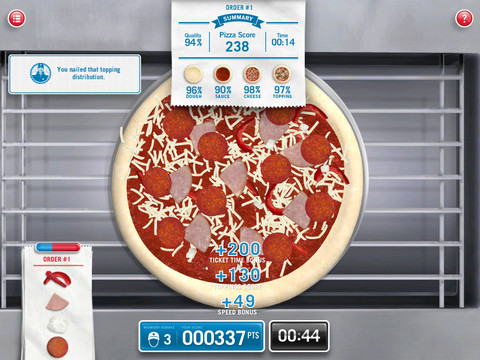
\includegraphics[width=\textwidth]{Figures/domino.png}
	\caption{نمایی از بازی قهرمان پیتزا دومینو \cite{domino}}
\end{figure}

\section{مدیریت عمل‌کرد و مشارکت}
قسمتی دیگر از فرایند مدیریت منابع انسانی بحث مدیریت عمل‌کرد و مشارکت است. سازمان‌های باید بتوانند نحوه کارکرد کارمندان را شناسایی کنند، آن را بهبود بخشند و در عمل‌کرد بین آن‌ها مشارکت ایجاد کنند \cite{review}.

برای ایجاد مشارکت بین کارمندان باید میزان رضایت شغلی افراد سنجیده شود. رضایت شغلی مبتنی بر ارزش‌ها و باورهای افراد شکل می‌گیرد و باید این موارد در فرایند ایجاد رضایت در افراد، در نظر گرفته شوند. زمانی که رضایت شغلی ایجاد می‌شود، کارمندان تمایل پیدا می‌کنند که به صورت خودجوش به تبلیغ سازمان بپردازند و مروجان سازمان باشند؛ بنابر این هنگام افزایش رضایت شغلی در کارمندان، علاوه بر بهبود عمل‌کرد کارمندان و ایجاد مشارکت، مزیت تبلیغ سازمان نیز رخ می‌دهد \cite{rezayat}.

طبق مطالعات چو \cite{actionable} گاهی مشارکت نتیجه مطلوبی ندارد و ایجاد رقابت بین کارمندان بهتر است. پیاده‌سازی روش‌های بازی‌وارسازی برای ایجاد مشارکت بین کارمندان و بهبود عمل‌کرد آن‌ها، مثل سایر قسمت‌ها نیازمند این است که جامعه بازیکنان سنجیده شود. در جامعه‌ای مثل ایران که فقر بازی به چشم می‌خورد و البته اکثر افراد از دسته قاتل‌ها هستند، این احتمال وجود دارد که بازی‌های مشارکتی و همکارانه مورد استقبال قرار نگیرند چون دید مناسب و مثبتی نسبت به این نوع بازی‌ها وجود ندارد \cite{atoz}. با استفاده از پرسش‌هایی که از افراد صورت می‌گیرد و تست‌های شخصیت به اضافه نگاه به فرهنگ سازمانی می‌توان دریافت که برای بهبود عمل‌کرد بین کارمندان بهتر است که رقابت ایجاد شود، مشارکت افزایش یابد یا ترکیبی از این دو در نظر گرفته‌شود \cite{reghmosh}.
\subsection{شبکه‌های اجتماعی کارمندان}
\label{sec:socialnetwork}
شبکه‌های اجتماعی سازمانی نوعی از شبکه‌های اجتماعی هستند که در آن افراد به تولید محتوای مرتبط با سازمان، دنبال‌کردن دیگر کارمندان و آشناشدن با دیگران (گسترش شبکه بین افراد) و اصلاح یا امتیازدهی به محتوای تولیدی دیگران می‌پردازند. بر اساس امتیازاتی که به محتواها داده می‌شود یک جدول برندگان تشکیل می‌شود و افراد رتبه‌بندی می‌شوند \cite{sharepoint}.
این شبکه‌های اجتماعی که عنصرهای مختلف بازی‌وارسازی را در خود به خوبی پیاده‌سازی می‌کنند علاوه بر ایجاد مشارکت به خاطر گسترش شبکه آشنایان کارمندان و همچنین ایجاد رقابت به دلیل مقایسه خود با دیگران، به سازمان‌ها کمک می‌کند که مدیریت دانش خوبی ایجاد کنند که این به بهبود عمل‌کرد آنان کمک می‌کند و البته تاریخچه‌ای نسبت به سازمان، اعضای سازمان و محتواهای تولیدشده مرتبط با اعضای فعلی و قدیمی سازمان برای کارمندان آینده جمع‌آوری می‌شود که در آموزش آن‌ها کمک‌کننده خواهد بود.

\begin{figure}[!htb]
	\centering
	\begin{minipage}[b]{0.49\textwidth}
		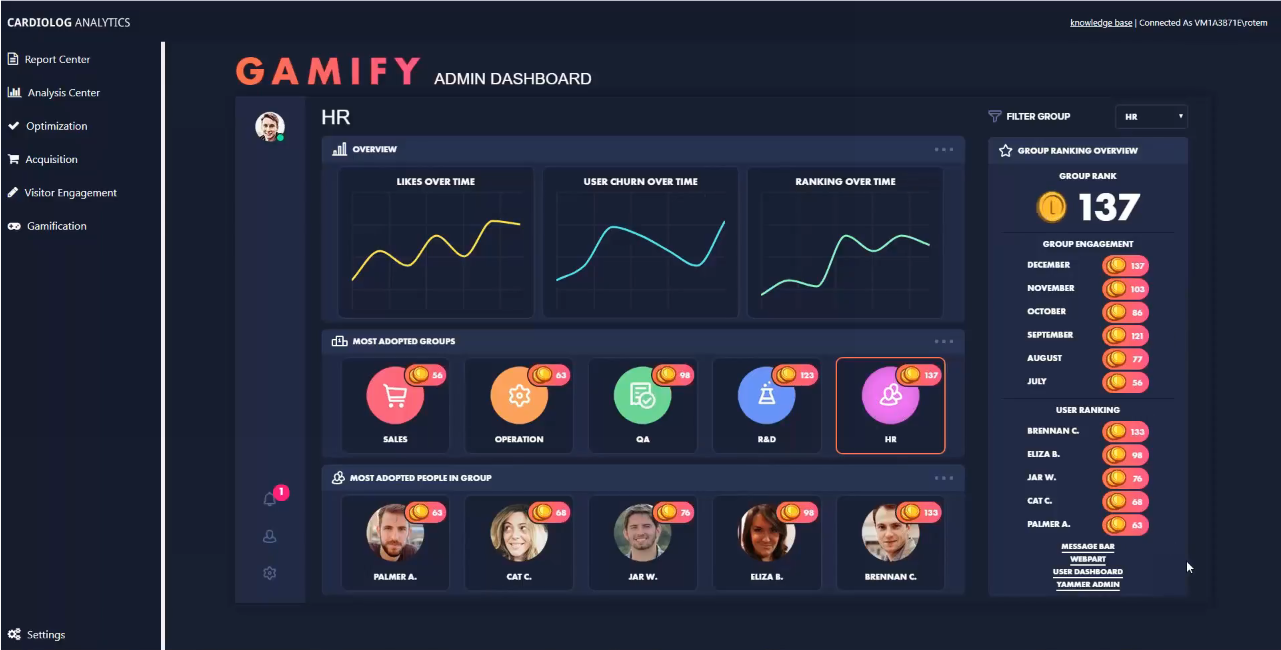
\includegraphics[width=\textwidth]{Figures/social1.png}
	\end{minipage}
	\begin{minipage}[b]{0.49\textwidth}
		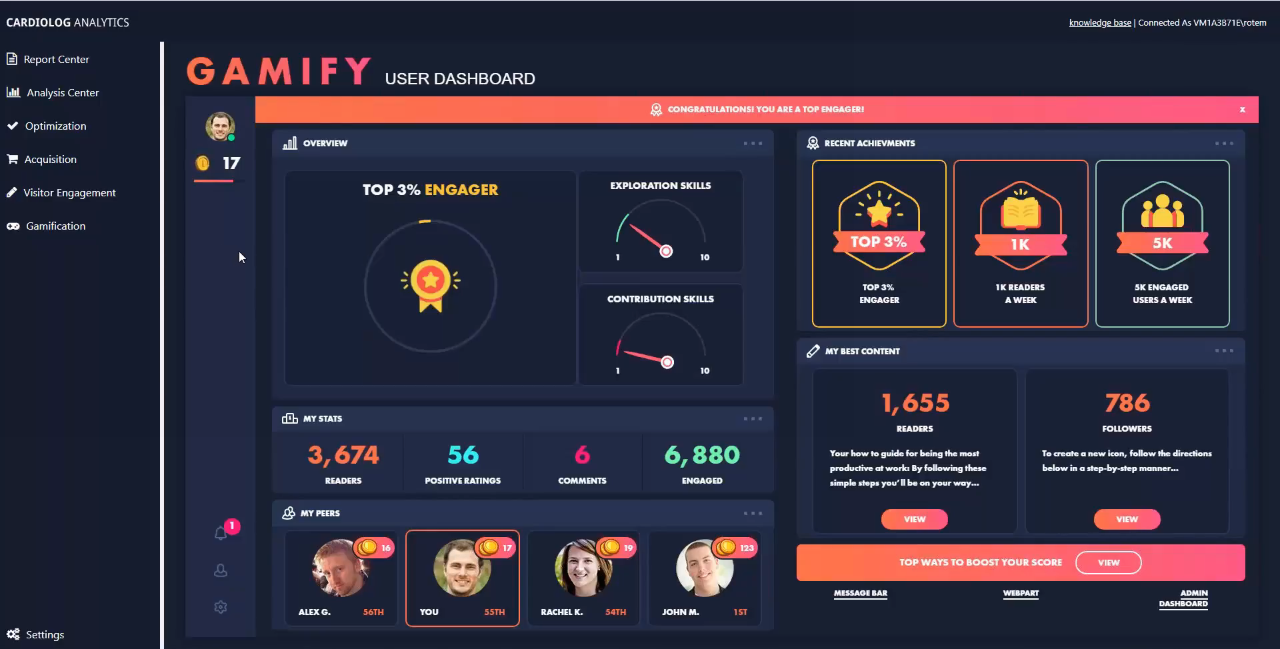
\includegraphics[width=\textwidth]{Figures/social2.png}
	\end{minipage}
	\caption{نمایی از شبکه اجتماعی مخصوص کارمندان یک سازمان\cite{sharepoint}}
\end{figure}

\subsection{بازی‌هایی برای بهبود جلسه‌های اداری}
در یک سخنرانی تد \cite{tedx} در مورد سازمانی صحبت شد که در تشکیل جلسه‌های سازمان، مشکلاتی مثل دیرکرد افراد، همهمه حین صحبت و طول‌کشیدن بیهوده زمان جلسه‌ها، وجود داشت و به همین خاطر سازمان سعی کرد با استفاده از سه ترفند به وضعیت جلسه‌ها نظم و کارآمدی را اضافه کند.
\begin{trick}[تیر هوایی]
هنگامی که جلسه شروع می‌شود، یک صدای بلند (می‌تواند شلیک هوایی واقعی باشد) در سازمان پخش می‌شود. این صدا به همه اعلام می‌کند که جلسه شروع شده‌است.
\end{trick}
\begin{trick}[ساعت جادویی]
یک ساعت خاص در جلسه وجود دارد که دقیقا روی ۱۵ دقیقه تنظیم شده‌است. زمانی که جلسه شروع شود، زمان‌سنج ساعت به جریان می‌افتد و سر ۱۵ دقیقه بعد، زنگ می‌زند. به این ترتیب جلسه طولانی نمی‌شود و در زمان مقرر پایان می‌یابد.
\end{trick}
\begin{trick}[پرندگان خشمگین\LTRfootnote{Angry birds}]
کسی که در حال صحبت است یک عروسک از بازی موبایلی پرندگان خشمگین در دست دارد؛ در حقیقت مجوز صحبت‌کردن برای هر کس این است که عروسک در دست او باشد. هنگامی که صحبت فرد پایان می‌یابد، عروسک را به طرف کسی که تمایل دارد صحبت کند، پرتاب می‌کند. به این شکل از همهمه در جلسات جلوگیری می‌شود و صحبت‌ها به نوبت انجام خواهند شد.
\end{trick}
\section{آموزش و استعداد}
بین آموزش و بهره‌وری ارتباط مستقیمی وجود دارد؛ به این شکل که هر مقدار در آموزش سرعت بالاتری داشته باشیم، در عمل‌کرد کارمندان شاهد بهبود بهره‌وری خواهیم بود. در این قسمت می‌توانیم از راهکارهای مرتبط با بازی‌وارسازی در آموزش استفاده کنیم که به چند مورد از آن‌ها در ادامه پرداخته می‌شود \cite{amiriamin}.
\subsection{اتاق فرار}\LTRfootnote{Escape room}
اتاق فرار یک بازی فیزیکی است که شامل یک اتاق و چند نفر زندانی است. زندانی‌ها باید با حل معماها و چالش‌های درون اتاق، راه فرار را پیدا کنند و خودشان را نجات دهند. این معماها و چالش‌ها در اکثر مواقع باید به صورت همکارانه حل شوند، گاهی به تحلیل علمی نیاز دارند و در بعضی از مواقع متکی به هوش خواهند بود \cite{atoz}.

استفاده از اتاق فرار برای آموزش می‌تواند به طراحان بازی کمک کند که توانایی علمی افراد را بسنجند و استعدادهای نهفته‌ی افراد را آشکار کنند. مثلا اگر فردی قدرت رهبری خوبی داشته باشد، در این بازی توانایی خود را به خوبی نشان می‌دهد.
\subsection{موشک تک‌دستی}
یک بازی ساده است که در آن افراد باید موشک‌های کاغذی درست کنند و یک قانون دارد! قانون بازی این است که هیچ‌کس حق ندارد از دو دست خود استفاده کند؛ یعنی، افراد باید تنها با یک دست موشک بسازند. بدیهی است که ساخت موشک صرفا با یک دست کاری سخت و حتی ناشدنی است، به همین خاطر، افراد نیاز پیدا می‌کنند که با مشارکت یکدیگر موشک را بسازند و در حقیقت دو دست از دو نفر برای ساخت موشک تشکیل داده شود \cite{tedx}.

زمانی که کارمندان شرکت در اتاق انتظار قرار دارند یا در حال سپری کردن وقتی آزاد هستند، به آن‌ها این بازی پیشنهاد داده می‌شود. این بازی به کارمندان آموزش می‌دهد که چگونه با یکدیگر تعامل کنند و درصد مشارکتشان بالاتر برود.
\section{مدیریت دانش}
مدیریت دانش هم به آموزش سریع‌تر کمک می‌کند و هم در عمل‌کرد افراد فعلی و آینده سازمان موثر است چراکه راه‌های پیموده‌شده برای حل مسائل را به آن‌ها نشان می‌دهد. مدیریت دانش به عنوان یکی از مهم‌ترین کارهای سازمان و البته در حین فرایند مدیریت منابع انسانی، نیازمند داشتن مشارکت خوبی بین کارمندان است. در سازمان دانش ارزشمند است \cite{kmanagement} و با وجود مشارکت بین اعضا می‌توان به بهبود دانش افراد و در نتیجه مدیریت دانش، دست پیدا کرد. بازی‌وارسازی با راهکارهایی مثل شبکه اجتماعی کارمندان (رجوع شود به زیربخش \ref{sec:socialnetwork}) می‌تواند در فرایند مدیریت دانش به سازمان کمک کند و انجام آن را تسریع کند \cite{amiriamin}.
\subsection{شرکت مشاوره‌ای \lr{Blue wolf}}
به نقل از \cite{modiran}، شرکت \lr{Blue wolf} با استفاده از روش‌های بازی‌وارسازی سعی کرد فرایند مدیریت دانش در سازمان را بهبود دهد؛ به همین خاطر در اولین اقدام \emph{بلندگو را به همه کارمندان داد} و از نشت اطلاعات سازمان جلوگیری نکرد. برای هر فرد در سایت این شرکت، یک صفحه شخصی یا یک صفحه گروهی (با مشارکت گروهی از کارمندان) وجود دارد که بر روی آن افراد به تولید محتوا می‌پردازند. از سمت سازمان برای تولید محتوا، امتیازها و نشان‌هایی در نظر گرفته می‌شود که به افراد اعطا می‌شود. این کارها باعث شد در تولید محتوا خلاقیت ایجاد شود و اعضا با مشارکت یکدیگر به فرایند مدیریت دانش کمک کنند. از سمت دیگر به خاطر انتقال دانش سازمان به بیرون از آن، به شهرت این شرکت افزوده شد و کارمندان آن اعتبار بیشتری پیدا کردند که این سبب شد مشاوران شرکت نسبت به گذشته ۵۷ درصد بیشتر فعالیت داشته باشند \cite{bluewolf}. در نهایت به خاطر افزایش دانش و اعتبار شرکت، دارایی‌های شرکت افزایش پیدا کرد.

\begin{figure}[!htb]
	\centering
	
\includegraphics[width=\textwidth]{Figures/goingsocial.jpg}
	\caption{نمایی از سایت شرکت \lr{Blue wolf} \cite{goingsocial}}
\end{figure}

\section{فرهنگ سازمانی}
در بحث فرهنگ سازمانی مجددا دانش، مشارکت و مدیریت این موارد مطرح می‌شود اما فرهنگ باید در افراد نهادینه شود. هر میزان که نهادینه‌سازی فرهنگ در افراد سریع‌تر باشد، عمل‌کرد افراد و توانایی مشارکت بین آن‌ها افزایش پیدا می‌کند. لازمه انتقال فرهنگ، انتقال آگاهی است. این کار با استفاده از یک بازی سازمانی مبتنی بر بازی جومانجی\LTRfootnote{Jumanji} قابل انجام است \cite{amiriamin}.
\subsection{مدل بازی جومانجی}
بازی جومانجی یک بازی رومیزی\LTRfootnote{Boardgame} است که در آن هر شخصیت دارای یک قدرت ویژه است  که با این قدرت‌ها باید با خود بازی مبارزه کنند تا همه پیروز از بازی خارج شوند. این مدل در سایت مسترگیمیفیکیشن \cite{jumanji} مطرح شده‌است.

یک بازی سازمانی بر اساس این بازی می‌توان ساخت که در آن بازیکنان افراد تازه‌وارد به سازمان هستند، هر کدام از آن‌ها یک قدرت خاص دارند و هدف یافتن مدبرعامل است. در اولین روز کاری، قبل از شروع بازی تمام امکاناتی که به کارمندان تازه‌وارد در تقلب‌کردن کمک می‌کند (مثل تلفن همراه یا لپتاپ) از آن‌ها گرفته می‌شود. قدرت‌های خاص بازیکنان می‌تواند توانایی مصاحبه با بخش بازاریابی، استفاده محدود از تلفن همراه یا موارد دیگر باشد که با مشارکت بین افراد و جمع‌شدن قدرت‌ها افراد می‌توانند به هدف بازی یعنی یافتن مدیر عامل برسند.

هنگامی که مدیرعامل پیدا می‌شود، اعضای تازه‌وارد با مدیرعامل جشن می‌گیرند و به یک مهمانی دعوت می‌شوند. 
این بازی باعث می‌شود افراد تازه‌وارد به سرعت با فرهنگ سازمانی و محیط شرکت آشنا شوند، با دیگر افراد سازمان آشنا شوند و شبکه آن‌ها گسترش پیدا کند و البته نسبت به یکدیگر درک بیشتری پیدا می‌کنند. به علاوه این موارد باعث می‌شود که افراد خاطره خوبی از اولین روز کاری خود در سازمان داشته باشند و حتی در صورتی که سازمان را ترک کنند، این خاطره از ذهن آن‌ها پاک نمی‌شود.

% % !TEX root = ../gamification-in-human-resource-management.tex
% !TeX program = xelatex
\chapter{نتیجه‌گیری}
در این نوشتار راجع به این موضوع که چطور می‌توانیم در فرایند مدیریت منابع انسانی از روش‌های بازی‌وارسازی استفاده کنیم، بحث شد. ابتدا مفاهیم اولیه‌ای در ارتباط با بازی، بازیکن، بازی‌وارسازی و فرایند مدیریت منابع انسانی ارائه شد و پس از آن کارهایی که تا کنون در ارتباط با این فرایند انجام شده‌اند، بررسی شدند.
% \input{Chapters/Chapter4}
% \input{Chapters/Chapter5}
% \input{Chapters/Chapter6}

% === References ===
% \MakeReferences{References}

% === Re-Style ===
% \clearpage
\pagestyle{myheadings}
% \pagenumbering{arabic}
% \setcounter{page}{1}

% === Chapters ===
% \clearpage
% \baselineskip=0.9cm
\linespread{1.0} % single-line spacing
% \linespread{1.3} % one and a half line spacing
% \linespread{1.6} % double-line spacing

\settextfont[Scale=1.2, ItalicFont=*, ItalicFeatures={FakeSlant=0.32}, BoldItalicFont=* Bold, BoldItalicFeatures={FakeSlant=0.32}]{B Nazanin}
\titleformat{\chapter}[display]
{\fontsize{15pt}{0}\selectfont  \flushleft  \bfseries \BNazaninScaleOne} % B Nazanin 15
{\chaptertitlename\ \tartibi{chapter}}{0.3cm}{\fontsize{15pt}{0}\selectfont \BNazaninScaleOne} % B Nazanin 15

\sectionfont{\fontsize{14pt}{\baselineskip}\selectfont \bfseries \BNazaninScaleOne} % B Nazanin 14
\subsectionfont{\fontsize{13pt}{\baselineskip}\selectfont \bfseries \BNazaninScaleOne} % B Nazanin 13
\subsubsectionfont{\fontsize{13pt}{\baselineskip}\selectfont \bfseries \BNazaninScaleOne} % B Nazanin 13

\titlespacing*{\section}{0pt}{1.2\baselineskip}{0pt}
\titlespacing*{\subsection}{0pt}{1.1\baselineskip}{0pt}
\titlespacing*{\subsubsection}{0pt}{1\baselineskip}{0pt}

\makeatletter
\renewcommand\chapter{\if@openright\cleardoublepage\else\clearpage\fi
	\global\@topnum\z@
	\@afterindentfalse
	\secdef\@chapter\@schapter}
\makeatother

% === Appendices ===
% \MakeAppendices
\captionsetup{list=no}
% \input{Chapters/Appendices}

% === Dictionary ===
\onehalfspacing
% \input{Chapters/dicfa2en}
% \input{Chapters/dicen2fa}
% \input{Chapters/acronyms}

% === English Abstract ===
% \input{Chapters/AbstractEn}
% \MakeEnglishAbstract

% === English Signature ===
\DepartmentEn{Faculty of Computer Engineering}
\DegreeEn{Ph.D.} % Or \DegreeEn{M.Sc.)} 
\YourFullnameEn{Student First and Last Name}
\DateEn{Month Year} %
\FirstSupervisorEn{Supervisor First and Last Name}
\TitleEn{Thesis English Title} 
\GroupEn{Department of Software Engineering}
\FirstAdvisorEn{First Advisor, Assoc. Prof.}
% \MakeEnglishSignaturePage

\end{document} 
